\documentclass[a4paper,12pt]{article}

\title{Introduktion til programmering, ugeseddel 3}
\author{Version 1.0}% Martin Dybdal
\date{13.\ september 2014}

\usepackage{cmap}
\usepackage[top=2cm,left=25mm]{geometry}
\usepackage[T1]{fontenc}
\usepackage[utf8]{inputenc}
\usepackage[danish]{babel}
%\usepackage{microtype}
\hyphenpenalty=750

\usepackage{amsmath}
%\usepackage{lmodern}
%\usepackage{mathptmx}
%\usepackage{libertine}
%\usepackage[scaled=0.90]{inconsolata}
%\usepackage[scaled=0.83]{beramono}

\usepackage{enumerate}
\usepackage{listing}
\usepackage{fancyvrb}
\usepackage{graphics,tikz}
\usepackage{listings}

\lstset{
    language=ML,
    keywordstyle=\bfseries,
    showstringspaces=false,
    basicstyle=\footnotesize\ttfamily,
    %numberstyle=\footnotesize,
    %numbers=left,
    %stepnumber=1,
    numbersep=10pt,
    tabsize=2,
    breaklines=false,
    aboveskip={0.7\baselineskip},
    columns=fixed,
%    extendedchars=true
% frame=single,
% backgroundcolor=\color{lbcolor},
}

\usepackage{todonotes}


\usepackage{hyperref}
\hypersetup{pdftitle={Introduktion til programmering, ugeseddel 3},
            pdfsubject={},
            pdfauthor={},
            pdfkeywords={rekursion, funktioner, lister, funktioner som værdier, højereordensfunktioner},
            pdfborder={0 0 0}}

\setlength{\parskip}{1ex}
\setlength{\parindent}{0pt}
\setlength{\parfillskip}{30pt plus 1 fil}

\makeatletter
\newcommand\footnoteref[1]{\protected@xdef\@thefnmark{\ref{#1}}\@footnotemark}
\makeatother


\begin{document}
\maketitle{}
Den tredje undervisningsuge har til formål at gøre jer fortrolige med
brug af funktioner som \textit{værdier}. Ind til nu har vi adskilt
funktioner fra primitive typer af værdier (f.eks. heltal og
sandhedsværdier), men som vi vil se i denne uge kan funktioner også
gemmes i lister, funktioner kan gives som argumenter til andre
funktioner, og en funktion kan "`konstruere"' andre funktioner.

Derudover skal vi lære hvordan vi med \textit{lokale erklæringer} kan
give navne til mellemresultater i en funktion, og hvordan vi kan bruge
det til at skjule hjælpefunktioner.

\section{Plan for ugen}
\label{sec:pensum-og-plan}

\subsubsection*{Mandag}
Lokale erklæringer, funktioner som værdier og introduktion til
ugesedlens tema.

\textit{Pensum:} HR: 3.7 $\rightarrow$ IP-2: 4.5 $\rightarrow$
\texttt{\footnotesize 3M-kvadratrod2-local.sml}\footnote{\label{seeabsalon} Findes på Absalon} $\rightarrow$ IP-2:
10.1-10.2

\subsubsection*{Tirsdag}
Listekombinatorer, anonyme funktioner og virkefelter.

\textit{Pensum:}\\ IP-2: 10.3-10.5 $\rightarrow$ HR: 9.1-9.5.1 og 9.6 $\rightarrow$ \textit{Intuition for \texttt{foldl}}\footnoteref{seeabsalon}

\subsubsection*{Fredag}
\texttt{foldl} vs. \texttt{foldr} og effektiv sortering

\textit{Pensum:} HR: 9.5.2 $\rightarrow$ IP-2: 8

\newpage
\section{Opgavetema: Programmering med billeder}
% Forklar: beside, clockwise, scale, RGB og recolour, transform,
%          koordinatsystem, blankImage, RGB.<farve>
% readBMP/writeBMP
I denne uge skal I lære om hvordan funktioner kan bruges som værdier,
til det formål har vi skrevet et lille SML-bibliotek til at manipulere
billeder. I denne sektion vil vi forklare hvordan det bruges. Vi vil
bruge billedet "torben.bmp" som udgangspunkt:
\begin{figure}[h!]
  \centering
  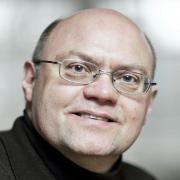
\includegraphics[width=3cm]{uge3_torben.png}

  \caption{torben.bmp}
\label{fig:torben}
\end{figure}

Start med at indlæse biblioteket:
\begin{lstlisting}
    use "InstagraML.sml";
\end{lstlisting}

Nu kan vi indlæse en billedfil\footnote{Billeder skal være i bitmap-formattet
  (dvs. "`.bmp"'-filer). Du kan konvertere billeder online vha.
  \url{http://www.imagemagick.org/MagickStudio/scripts/MagickStudio.cgi}}
fra harddisken (kun BMP, se fodnote):
\begin{lstlisting}
    val torben = InstagraML.readBMP "torben.bmp";
\end{lstlisting}

Det simpleste vi kan gøre ved et billede er at rotere det
90$^\circ$ i urets retning:
\begin{lstlisting}
    val torbenPaaSiden = InstagraML.clockwise torben;
\end{lstlisting}
For at se resultatet skal vi gemme billedet til en ny fil:
\begin{lstlisting}
    - InstagraML.writeBMP ("torbenPaaSiden.bmp", torbenPaaSiden);
    > val it = () : unit
\end{lstlisting}
Vi kan nu finde filen \verb|torbenPaaSiden.bmp| på harddisken:

\begin{figure}[h!]
  \centering
  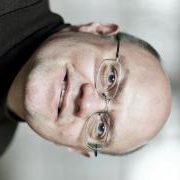
\includegraphics[width=3cm]{uge3_torbenPaaSiden.png}

  \caption{torbenPaaSiden.bmp}
\label{fig:torbenPaaSiden}
\end{figure}

Bemærk typen af \verb|writeBMP|:
\begin{lstlisting}
    InstagraML.writeBMP : string * image -> unit
\end{lstlisting}
Returværdien er værdien \verb|()|, da det ikke er selve resultatet af
funktionen vi er interesseret i, men at den laver en ændring på vores
harddisk.

\subsection*{Farver og \texttt{colour}-typen}
For at forstå hvad et billede er, skal vi vide hvordan en computer
"`regner"' med farver. En farve er en blanding af rød, grøn og blå
farve. I SML repræsenterer vi blandingsforholdet mellem de tre farver
som en trippel bestående af tre heltal mellem 0 og 255.

\noindent
\textbf{Eksempel:}
\begin{lstlisting}
    val red     = (255,  0,  0);
    val green   = (  0,255,  0);
    val blue    = (  0,  0,255);
    val magenta = (255,  0,255);  (* magenta = bland roed og blaa *)
\end{lstlisting}

Vi har introduceret typeforkortelsen \verb|colour| for at gøre typerne
nemmere at læse. At skrive \verb|colour| betyder altså præcist det
samme som at skrive \verb|int * int * int|. MosML vil dog blive ved
med at skrive \verb|int * int * int| når den udskriver typerne.

\subsection*{Hvad er et billede?}
Et billede er en angivelse af hvilken farve, hver enkelt lille punkt på
billedet har. Hvert sådan et punkt kaldes en pixel. Billedet af Torben
der er blevet brugt ovenfor er $180$ pixels i bredden og $180$ pixels
i højden, dvs. at der er $180 \times 180 = 32400$ pixels i
billedet. For hver af disse punkter skal der gemmes en farve.

Vi behøver i denne opgave ikke præcist at vide hvordan et billede
gemmes på harddisken, men blot at \verb|readBMP| og \verb|writeBMP|
gør det for os.

\noindent

\textbf{Eksempel:} For at lave et billede hvor alle pixels har samme
farve kan vi bruge funktionen \verb|InstagraML.pixel|, der givet en
farve returnerer et billede med størrelse $1 \times 1$. Hvis man har
behov for det kan man skalere 1-pixel billedet til de ønskede
dimensioner. Se \verb|InstagraML.scale| nedenfor.

\begin{lstlisting}
  - InstagraML.writeBMP ("green.bmp", InstagraML.pixel green);
  > val it = () : unit
\end{lstlisting}
\begin{figure}[h!]
  \centering
  
\includegraphics[width=5cm]{uge3_green.png}

  \caption{green.bmp skaleret til størrelse 512x512 pixels}
\label{fig:green}
\end{figure}


\newpage
\subsection{InstagraML dokumentation}
Til at starte med behøver I ikke forstå alt i denne sektion, gå i
stedet i gang med opgaverne og slå op her undervejs.
\subsubsection*{\texttt{pixel : colour -> image}}
\begin{quotation}
\noindent
Returnerer et billede med 1 pixel i bredden og 1 pixel i højden, af
den angivne farve.
\end{quotation}

\subsubsection*{\texttt{width : image -> int} }\vspace{-5mm}
\subsubsection*{\texttt{height : image -> int}}
\begin{quotation}
\noindent
Returnerer henholdsvis bredden og højden af billedet i antal af pixels.

\vspace{1em}
\noindent
\textbf{Eksempel:}
\begin{lstlisting}
  - InstagraML.width torben;
  > val it = 180 : int
  - InstagraML.height (InstagraML.pixel green);
  > val it = 1 : int
\end{lstlisting}
\end{quotation}

\subsubsection*{\texttt{clockwise : image -> image}}
\begin{quotation}
\noindent
Roterer et billede 90$^\circ$ i urets retning.

\vspace{1em}
\noindent
\textbf{Eksempel:} \lstinline{InstagraML.clockwise torben;}
\begin{figure}[h!]
  \centering
  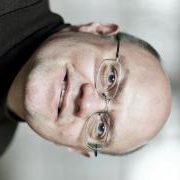
\includegraphics[width=3cm]{uge3_torbenPaaSiden.png}
\end{figure}
\end{quotation}

\subsubsection*{\texttt{beside : image * image -> image}}
\begin{quotation}
\noindent
Sætter to billeder ved siden af hinanden.

\vspace{1em}
\noindent
\textbf{Eksempel:} \lstinline{InstagraML.beside (torben, torben);}
\begin{figure}[h!]
  \centering
  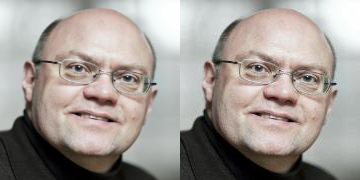
\includegraphics[width=6cm]{uge3_torbenBesideTorben.png}
\end{figure}
\end{quotation}

\subsubsection*{\texttt{scale : real -> real -> image -> image}}
\begin{quotation}
\noindent
Skalerer størrelsen af et billede. Det første argument ganges på
bredden af billedet, det andet argument ganges på højden af billedet.

\vspace{1em}
\noindent
\textbf{Eksempel:} \lstinline{InstagraML.scale 2.0 0.5 torben;}
\begin{figure}[h!]
  \centering
  
\includegraphics[width=6cm]{uge3_scaleTorben.png}
\end{figure}
\end{quotation}

\subsubsection*{\texttt{recolour : (colour -> colour) -> image -> image}}
\begin{quotation}
\noindent
Vi kan aflæse af typen af recolour at dens første argument er en
funktion der ændrer en '\verb|colour|' til en anden
'\verb|colour|'. Idéen er at vi kan "`omfarve"' et billede ved at give
en funktion der fortæller hvordan farven af hver pixel skal ændres.

\vspace{1em}
\noindent
\textbf{Eksempel:}
\begin{lstlisting}
(* Goer et billede mere blaat (mere brugervenligt) *)
fun makeBlue (r,g,b) = (r,g,255);
val blueTorben = InstagraML.recolour makeBlue torben;
\end{lstlisting}
\begin{figure}[h!]
  \centering
  
\includegraphics[width=3cm]{uge3_blaaTorben.png}
\end{figure}
\end{quotation}

% \subsubsection*{\texttt{transform : (real*real -> real*real) -> image -> image}}
% \begin{quotation}
% \noindent
% Ved et kald \verb|transform f img| er første argumentet \verb|f| en
% funktion der fortæller hvor pixels i det nye billede skal aflæses i
% det gamle. For hver pixel i det billede der skal konstrueres kaldes
% \verb|f| og \verb|f| returnerer så et koordinat i det gamle billede,
% hvorfra farven tages. Hvis \verb|f| returnerer et koordinat der peger
% uden for det gamle billede, sættes den pågældende pixel i det nye
% billede til sort.

% \vspace{1em}
% \noindent
% \textbf{Eksempel:} I filen \verb|Effects.sml| findes funktionen
% \verb|whirl|.

% \begin{lstlisting}
% InstagraML.transform whirl torben;
% \end{lstlisting}
% \begin{figure}[h!]
%   \centering
%   
\includegraphics[width=3cm]{uge3_whirlTorben.png}
% \end{figure}
% \end{quotation}

% \todo[inline]{forbedr forklaring af transform}


\subsection{Afprøvning}
Opgaverne til denne uge der omhandler InstagraML-billeder er
afprøvning ikke helt så lige til. Det er svært at konstruere det
forventede output og InstagraML har pt. ikke en funktion til at
sammenligne to billeder. Vi forventer derfor at en del af jeres
afprøvning beror på \textit{visuel inspektion} af
resultaterne.

To ting er det dog muligt at skrive testtilfælde for: at de
resulterende billeder har de forventede dimensioner og at jeres
funktioner kaster undtagelser på de tidspunkter det er specificeret i
opgaveteksten.

\newpage
\section{Mandagsopgaver}
\label{sec:mandagsopgaver}
Mål: Blive endnu bedre til rekursion over lister. Intro til InstagraML
biblioteket.


\textit{De følgende opgaver løses vha. funktionerne gennemgået i
  afsnit 2.1. Ingen af opgaverne i denne uge kræver at I forstår eller
  redigerer hvad der sker internt i InstagraML.sml}


\begin{enumerate}[{3}M1]
\item I denne opgave skal du skrive en funktion der summerer de tal i
  en liste der opfylder et givent kriterie. Som eksempel bruger vi
  kriteriet at \textit{tallet skal være positivt}:
\begin{lstlisting}
  fun isOkay x = x > 0
\end{lstlisting}

Skriv funktionen \verb|sumIfOkay : int list -> int| der summerer alle
de tal i listen hvor \verb|isOkay| returnerer \verb|true|. Afprøv med andre
definitioner af \verb|isOkay|.

\item HR 5.14

\item Skriv en funktion:
\begin{lstlisting}
  counterClockwise : image -> image
\end{lstlisting}
  Der roterer et billede 90$^\circ$ mod urets retning.

\item Skriv en funktion der placerer et billede oven på et andet,
  sådan så højden af det nye billede er summen af højden af de to
  argument-billeder. Første argument skal placeres over andet
  argument. Kast undtagelsen \verb|Domain| hvis to billeder er af
  forskellig bredde.
\begin{lstlisting}
  above : image * image -> image
\end{lstlisting}

% \item Skriv en funktion:
% \begin{lstlisting}
%   repeatHorizontal : int * image -> image
% \end{lstlisting}
%   Der gentager et billede $n$ gange ved siden af hinanden. Kast
%   undtagelsen \verb|Domain| i tilfældet hvor $n=0$.

\item Skriv en rekursiv funktion:
\begin{lstlisting}
  imageConcat : image list -> image
\end{lstlisting}
  Der sætter alle billederne i en liste ved siden af
  hinanden. Funktionen skal kaste undtagelsen \verb|Empty| hvis listen
  er tom. Tirsdag vil vi se hvordan imageConcat kan skrives uden brug
  af rekursion.

\item Omskriv \verb|counterClockwise| så den skrives uden brug af
  "\texttt{fun}", men som en værdierklæring.
\begin{lstlisting}
  val counterClockwise = ...
\end{lstlisting}
  Hint: brug funktionssammensætning $(f~\texttt{o}~g)$, forklaret i HR
  afsnit 9.6.
\end{enumerate}
\vspace{5mm}
Hvis du har mere tid, gå da i gang med at forberede dig til
tirsdagsøvelserne.

\newpage
\section{Tirsdagsopgaver}
\label{sec:tirsdagsopgaver}
Mål: Videre med InstagraML og brug af listekombinatorerne map, filter og foldl.

Det forventes, at du inden øvelserne tirsdag har forberedt dig på
opgaverne ved at løse så mange som muligt på egen hånd.
\begin{enumerate}[{3}T1]
\item Skriv en funktion der tager gennemsnittet af to farver
  (gennemsnittet af hvert komponent):
\begin{lstlisting}
  colourAverage : colour -> colour -> colour
\end{lstlisting}

\item Erklær en funktion der gør et billede rødere ved at for hver
  pixel tager gennemsnittet af dens nuværende farve og postkasserød,
  (255,0,0).
\begin{lstlisting}
  fadeRed : image -> image
\end{lstlisting}

\item
Overvej hvorfor vi ikke har givet \verb|colourAverage| typen:
\begin{lstlisting}
  colourAverage : colour * colour -> colour
\end{lstlisting}

\item Funktioner af typen \verb|image -> image| kalder vi effekter,
  find flere eksempler i \verb|Effects.sml|.

  Skriv en funktion \verb|iterate| der anvender den samme effekt $n$
  gange på et billede, og sætter alle mellemresultaterne ved siden af
  hinanden:
\begin{lstlisting}
  iterate : (image -> image) -> image -> int -> image
\end{lstlisting}

\textbf{Eksempel:} \lstinline{iterate fadeRed torben 5;}
\begin{figure}[h!]
  \centering
  
\includegraphics[width=15cm]{uge3_fadeTorben.png}
\end{figure}

\item Omskriv funktionen \verb|sumIfOkay| fra opgave 3M1, så
  \verb|isOkay| gives som et argument:
  \verb|sumIfOkay2 : (int -> bool) -> int list -> int|

\item Omskriv \texttt{imageConcat} fra 3M5, så den bruger \verb|foldr| i
  stedet for rekursion.

\item HR 9.2(a)

% \item Skriv en funktion:
% \begin{lstlisting}
%   repeat : (image * image -> image) -> image -> int -> image
% \end{lstlisting}


% \item Skriv en funktion vha. \verb|recolour|:
% \begin{lstlisting}
%   greyscale : image -> image
% \end{lstlisting}
% Der konverterer et billede til gråtoner. En grå farve er
% karakteriseret ved at bestå af lige meget rød, grøn og blå. Det eneste
% der bevares er intentiteten af farven. En (ikke helt korrekt) måde at
% finde intensiteten af en farve er at tage gennemsnittet af de tre
% farvekanaler.
\end{enumerate}

\newpage
\section{Gruppeaflevering}
\label{sec:gruppeaflevering}
Gruppeafleveringen obligatorisk.  Alle delspørgsmål skal besvares.
Opgaven afleveres i Absalon.  Der afleveres en fil pr.\ gruppe, men
den skal angive alle deltageres fulde navne i kommentarlinjer øverst i
filen. Filens navn skal være af formen
\texttt{3G-\textit{initialer}.sml}, hvor initialer er erstattet af
gruppemedlemmernes initialer. Hvis f.eks. Bill~Gates, Linus~Torvalds,
Steve~Jobs og Gabe~Logan~Newell afleverer en opgave sammen, skal filen
hedde \texttt{3G-BG-LT-SJ-GLN.sml}. Brug gruppeafleveringsfunktionen i
Absalon.

Gruppeopgaven giver op til 2 point, som tæller til de 20 point, der
kræves for eksamensdeltagelse.  Genaflevering kan hæve pointtallet fra
første aflevering med højest 1 point, så sørg for at gøre jeres bedste
allerede i første aflevering.

\vspace{1cm} Denne opgave handler om problemløsning, som det blev
gennemgået tirsdag i uge 2. Se noterne "`Hvordan man angriber et
programmeringsproblem"' på Absalon.

Funktionen \verb|InstagraML.beside| kan ikke håndtere at sætte to
billeder ved siden af hinanden, der ikke er lige høje. I gruppeopgaven
er det jeres opgave at skrive en funktion \verb|safeBeside| der
centrerer det laveste af de to billeder ved siden af det andet og
indsætter sort farve i det tomrum der opstår over og under det laveste
billede.

\vspace{5mm}
\textbf{Eksempel:} \verb|safeBeside ralf torben|
\begin{figure}[h!]
  \centering
  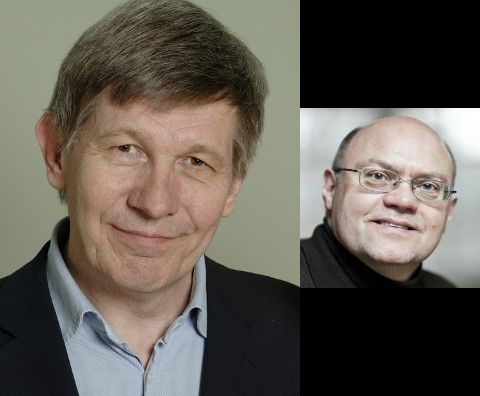
\includegraphics[width=5cm]{uge3_ralfTorben.png}
  \label{fig:safeBeside}
\end{figure}
\vspace{-5mm}

\begin{enumerate}[{3G}1]
\item \textit{Forstå problemet:} Skriv (i en kommentar) de forskellige
  tilfælde der skal håndteres og beskriv hvordan en løsning ser ud i
  hvert tilfælde. Tænk blandt andet over hvad der skal ske når et af
  billederne har et ulige antal pixels i højden og det andet har et
  lige antal.

\item \textit{Planlæg afprøvning:} Ud fra observationerne i opgave
  3G1, skriv en plan for hvordan I vil afprøve \texttt{safeBeside}.
\end{enumerate}

\textit{Opdel problemet i delproblemer:} Vi kan opdele problemet
  i tre:
  \begin{enumerate}[~~a)]
  \item En funktion der laver et ensfarvet billede af en specificeret
    bredde og højde.
\item En funktion der sætter en sort bjælke over og under et billede,
  så det opnår den ønskede størrelse.
\item Selve funktionen \verb|safeBeside|.
  \end{enumerate}


\begin{figure}[h!]
  \centering
\textbf{Eksempel:} \verb|padVertical 300 torben|\\
\vspace{2mm}
  
\includegraphics[width=3cm]{uge3_paddedTorben.png}
  \label{fig:padVertical}
\end{figure}

\begin{enumerate}
\item[3G3] \textit{Kommentarer før kode:} Vi har medvilje været lidt uklare
  om punkt (a) og punkt (b). Beskriv i en kommentar hvad de to
  funktioner skal gøre.

\item[3G4] \textit{Udfør planen, start med det nemme:} Skriv en funktion
  der udfører punkt (a) i planen:
  \begin{lstlisting}
    solid : colour -> int * int -> image
  \end{lstlisting}

\item[3G5] \textit{Udfør planen:} Skriv en funktion der udfører punkt (b) i planen:
  \begin{lstlisting}
    padVertical : int -> image -> image
  \end{lstlisting}
  Hvis heltallet der angiver den \textit{nye} højde er mindre end
  højden af billedet, skal funktionen rejse undtagelsen Domain. Det er
  kun meningen at funktionen skal kunne gøre et billede større, ikke mindre.

\item[3G6] \textit{Udfør planen:} Skriv funktionen
  \begin{lstlisting}
    safeBeside : image * image -> image
  \end{lstlisting}
  Der placerer to billeder ved sidan af hinanden og sørger for at det
  mindste midterjusteres i forhold til det andet
  vha. \verb|padVertical|.

% \item Skriv funktionen
%   \begin{lstlisting}
%     safeAbove : image * image -> image
%   \end{lstlisting}
%   Der placerer to billeder over hinanden og på samme måde sørger for
%   at det \textit{smalleste} centreres under eller over det andet.
\end{enumerate}


\newpage
\section{Individuel aflevering}
\label{sec:indiv-aflev}

Den individuelle opgave er obligatorisk.  Alle delspørgsmål skal
besvares.  Opgaven afleveres i Absalon som en fil med navnet
\texttt{3I-\textit{navn}.sml}, hvor \texttt{\textit{navn}} er
erstatttet med dit navn. Hvis du fx hedder Anders~A.~And, skal
filnavnet være \texttt{2I-Anders-A-And.sml}. Skriv også dit fulde navn
som en kommentar i starten af filen.

Den individielle opgave giver op til 3 point, som tæller til de 20
point, der kræves for eksamensdeltagelse.  Genaflevering kan hæve
pointtallet fra første aflevering med højest 1 point, så sørg for at
gøre dit bedste allerede i første aflevering.

\begin{enumerate}[{3I}1]
\item I filen \verb|Effects.sml| finder du en række effekter, alle med
  typen \verb|image -> image|. Skriv en rekursiv funktion der, en
  efter en, anvender alle transformationerne i en liste på et givet
  billedet og returnerer billedet hvor alle effekterne er anvendt. Den
  første effekt i listen anvendes først.

\begin{lstlisting}
  effects : (image -> image) list -> image -> image
\end{lstlisting}

\textbf{Eksempel:} \verb|effects [clockwise, fadeRed, fadeRed] torben|

\item Man kan også anse funktionen \texttt{effects} som en funktion
  der sætter effekter sammen og returnerer en ny effekt. Det er måske
  nemmere at se hvis vi opsætter typen på denne måde:
\begin{lstlisting}
  effects : (image -> image) list ->
            (image -> image)
\end{lstlisting}
Hvad udskriver MosML hvis du spørger om typen af \texttt{effects}?
\begin{lstlisting}
- effects;
\end{lstlisting}
Og hvorfor?

\item Vi kan repræsentere et klokkeslæt som antal minutter siden
  midnat. For eksempel svarer 120 til kl. 2:00, 0 er midnat og 1439 er
  kl. 23:59. Vi kan nu opskrive butikkers åbningstider som et par af
  to sådanne tidsangivelser:

  \begin{lstlisting}
  val openHours =
        [(16*60,  4*60, "La Luna Pizzaria"), (* 16:00- 4:00 *)
         ( 8*60, 22*60, "Netto"),            (*  8:00-22:00 *)
         ( 0, 23*60+59, "Steno Apotek")]     (*  0:00-23:59 *)
  \end{lstlisting}

  Skriv en funktion \verb|openStores xs t| der givet en liste af
  åbningstider \verb|xs|, og et tidspunkt \verb|t| returnerer alle de
  butikker der har åbent. Typesignatur:
  \begin{lstlisting}
  openStores : (int * int * 'a) list -> int -> 'a list
  \end{lstlisting}
  Undtagelsen \lstinline{Domain} rejses hvis $t$ eller et af
  tidspunkterne i $xs$ er ugyldigt.

  Husk at tage højde for at tidspunkter kan krydse midnat
  (e.g. kl. 16:00 til 4:30) og at skrive udførlig afprøvning af
  funktionen.
\end{enumerate}


%\newpage
\section{Ugens nød}
\label{sec:ugens-nod}
I denne uge er \textit{Ugens nød} en kreativ udfordring. Vinderen af
Ugens nød er den studerende der det program der producerer det
\textit{flotteste} billede i dimensionerne 512x512 pixels. I må
maksimalt skrive 20 linjer SML-kode, af maks 80 tegn per linje. Blanke
linjer og linjer kun med kommentarer fraregnes. Vi vil også se på
kvaliteten af selve koden: valg af navne, kommentarer og brug af
højereordensfunktioner frem for eksplicit rekursion.

Dommerkomitéen består alle undervisere og instruktorer på kurset.

Afleveringsfristen er den samme som for den individuelle opgave. I
skal både aflevere BMP-filen og SML-filen. Ved fredagsforelæsningen i
uge 4 kåres den bedste løsning, og vinderen får en lille præmie.
\end{document}

%%% Local Variables:
%%% mode: latex
%%% TeX-master: t
%%% End:
